
\subsection{Debiasing Results}
\tabref{t:templates1} gives results on OCCTMP. Two OCCTMP
examples are given in \tabref{t:templates2}. We see that
DensRay can mitigate the gender bias in BERT as measured by
diff: bias between predicting he/she drops by large margin
(e.g., for bert-base from 1.98 to 0.36). The table indicates
that DensRay outperforms the other two methods on OCCTMP.
Note that
the prediction probabilities of debiasing conceptor are
quite low for both ``he'' and ``she''. However,
in relative terms, ``he'' is still strongly favored compared
to ``she''.
\tabref{t:weat1} shows the results on association tests. The debiasing performance of the three methods are comparable.

\begin{table}[ht]
\centering
\footnotesize
\begin{tabular}{lccccc}
\hline
model & prob(he) & prob(she) & sum &diff & var\\
\hline
bert-base & 0.66 & 0.19 & 0.85 &1.98&1.39\\
bert-base-hard & 0.35 & 0.42 & 0.77&0.42&0.09\\
bert-base-conceptor & 0.18 & 0.11 & 0.28 & 0.68&0.26\\
bert-base-densray & 0.48 & 0.37 & 0.86&\textbf{0.36}&0.07\\
\hline
bert-large  & 0.63 & 0.19 & 0.82  &1.82&1.30\\
bert-large-hard & 0.40 & 0.23 & 0.63&0.69&0.30\\
bert-large-conceptor & 0.43 & 0.18 & 0.61 & 1.03&0.53\\
bert-large-densray  & 0.47 & 0.31 & 0.77&\textbf{0.49}&0.13 \\
\hline
\end{tabular}
\caption{\tablabel{t:templates1} BERT debiasing results on OCCTMP. \textit{bert-base} and \textit{bert-large} are the original models without debiasing. \textit{prob(he)} is
	the average probability predicted for \textit{he} as the [MASK] in OCCTMP. We also show the average sum probability $sum=prob(he)+prob(she)$ and \textit{var}, the variance of \textit{ diff}, for reference.}
\end{table}

\begin{table}[h]
	\centering
	\footnotesize
	\begin{tabular}{cl{|}cccc{|}cccc}
		\hline
		&&\multicolumn{4}{c|}{bert-base}&\multicolumn{4}{c}{bert-large}\\
		%\hline
		&&\multicolumn{2}{c}{WEAT}&\multicolumn{2}{c|}{SEAT}&\multicolumn{2}{c}{WEAT}&\multicolumn{2}{c}{SEAT}\\
		\hline
		category & model & d & p& d & p& d & p& d & p\\
		\hline
		C6 & without debiasing & 0.66 & 0.08 &1.04&$<$10$^{-2*}$& 1.57 & $<$10$^{-2*}$ &0.50&$<$10$^{-2*}$\\
		& hard debiasing& 0.15 & 0.38&\textbf{-0.08}&0.67& 0.80 & 0.06&0.07&0.35\\
		& debiasing conceptor & \textbf{0.07} & 0.46&0.77&$<$10$^{-2*}$ & 1.33 & $<$10$^{-2*}$&\textbf{0.06}&0.37\\
		&densray & 0.62 & 0.12&0.36&0.02$^{*}$ & \textbf{0.76} & 0.07&0.13&0.22\\
		\hline
		C7 & without debiasing & 0.60 & 0.11 &0.17&0.15 & -0.40 & 0.75 &0.38&0.01$^{*}$\\
		& hard debiasing & \textbf{-0.07} & 0.56&\textbf{-0.06}&0.64 & -0.51 & 0.83&0.38&0.01$^{*}$\\
		& debiasing conceptor & 0.54 & 0.14&-0.25&0.93 & -0.32 & 0.73&\textbf{-0.60}&0.99\\
		& densray & 0.09 & 0.45&-0.47&0.99 & \textbf{0.06} & 0.05&-0.73&0.99\\
		\hline
		C8& without debiasing & 0.78 & 0.08 &0.81&$<$10$^{-2*}$ & -0.60 & 0.87 &-0.30&0.95\\
		& hard debiasing & -0.29 & 0.68&\textbf{-0.10}&0.71 & 0.78 & 0.06&\textbf{-0.03}&0.56\\
		& debiasing conceptor & 0.62 & 0.14&0.50&$<$10$^{-2*}$& \textbf{0.12} & 0.39&0.30&0.94\\
		& densray & \textbf{0.03} & 0.47&0.41&0.01$^{*}$ & 0.20 & 0.33&-0.66&0.99\\
		\hline
	\end{tabular}
	\caption{\tablabel{t:weat1}
		BERT debiasing results on association tests. * shows significant gender bias.}
\end{table}

\subsection{Model Performance}
\tabref{t:glue1} shows that DensRay debiasing gets comparable results with
the original models on Wikitext-2 and GLUE tasks.
In most tasks on bert-base and all tasks on bert-large, DensRay performs better than hard debiasing, so DensRay affects model performance less.
Similarly, in most tasks on bert-base and all tasks but one
on bert-large, DensRay performs better than debiasing conceptor, so DensRay affects model performance less.
\begin{table*}[h]
\centering
\footnotesize
\begin{tabular}{l||c|cccccccccc}
%\hline
model & Wikitext-2&CoLA &SST-2&MRPC&STS-B&RTE&WNLI&GLUE avg\\
\hline\hline
		bert-base &3.77&49.15&92.09&85.86&82.66&62.82&52.11&70.78\\
bert-base-hard &3.95&45.53&\textbf{91.74}&82.48&\textbf{82.60}&63.54&\textbf{56.34}&70.37\\
bert-base-conceptor &4.46&\textbf{48.31}&91.43&84.08&81.37&59.57&\textbf{56.34}&70.18\\
bert-base-densray &\textbf{3.81}&48.04&\textbf{91.74}&\textbf{84.89}&82.43&\textbf{63.90}&53.52&\textbf{70.75}\\
\hline
bert-large &3.29& 47.93&94.90&89.30&87.60&70.10&65.10&75.82\\
bert-large-hard &3.85& 47.45&93.95&85.01&82.33&67.12&63.02&73.15\\
bert-large-conceptor &4.13&\textbf{49.44}&93.87&87.67&83.44&62.45&56.34&72.20\\
bert-large-densray &\textbf{3.35}& 48.91&\textbf{94.02}&\textbf{88.84}&\textbf{85.63}&\textbf{67.78}&\textbf{64.48}&\textbf{74.94}\\
%\hline
\end{tabular}
\caption{\tablabel{t:glue1}
Language modelling perplexity and GLUE tasks
performance. }
\end{table*}


\subsection{Examples}
In \tabref{t:templates2} we show two OCCTMP examples.
Again, densray works best as measures by diff.
The sum probabilities of ``he'' and ``she''
on the debiasing conceptor are around 0.5, indicating that
the
language model has lost part of its ability to predict that 
a pronoun is  likely to occur in the masked position.
\begin{table}[h]
	\centering
	\footnotesize
	\begin{tabular}{llcccc}
		\hline
		sentence & model & prob(he) & prob(she) &sum&diff\\
		\hline
		[MASK] is a & bert-base & 0.84 & 0.13&0.97&1.86\\
		professor.& bert-base-hard& 0.37 & 0.55&0.92&0.40\\
		& bert-base-conceptor& 0.28 & 0.23&0.51&{0.20}\\
		& bert-base-densray & 0.53 & 0.37&0.90&0.36\\
		\hline
		[MASK] is a & bert-base & 0.22 & 0.72&0.94&1.19\\
		dancer.  & bert-base-hard& 0.27 & 0.64&0.91&0.86\\
		& bert-base-conceptor& 0.20 & 0.33&0.53&0.50\\
		& bert-base-densray& 0.42 & 0.52&0.94&0.21\\
		\hline
	\end{tabular}
	\caption{\tablabel{t:templates2}
		OCCTMP examples with prediction probabilities.}
\end{table}


\subsection{Analysis}

\subsubsection{Debiasing on Attention Heads and Layers}
We now apply DensRay to the attention heads in BERT to debias on OCCTMP. The heatmap \figref{fig:heads} shows that the debiasing effect of one single attention head is not apparent, with diff scores all in [1.0,1.4]. Due to the lack of dimensions and the distribution of gender features in the attention heads, we chose to apply DensRay on layers as a debiasing method. We conclude that there is no single attention head that is responsible for processing gender information.

So far we have always applied DensRay to all BERT layers
simultaneously. \figref{fig:layersbase}  illustrates the effect of
debiasing a single  layer on our templates and the three
WEAT categories. We see that the debiasing effect is
stronger in layers 7--10 than in the other layers in
bert-base.
\enote{hs}{
It is shown that gender information is extracted and processed on BERT layers, especially the upper layers. delete?}
\begin{figure}[h]
	\centering
	\subfigure[attention heads]{
		\begin{minipage}[l]{0.5\linewidth}
			\centering
			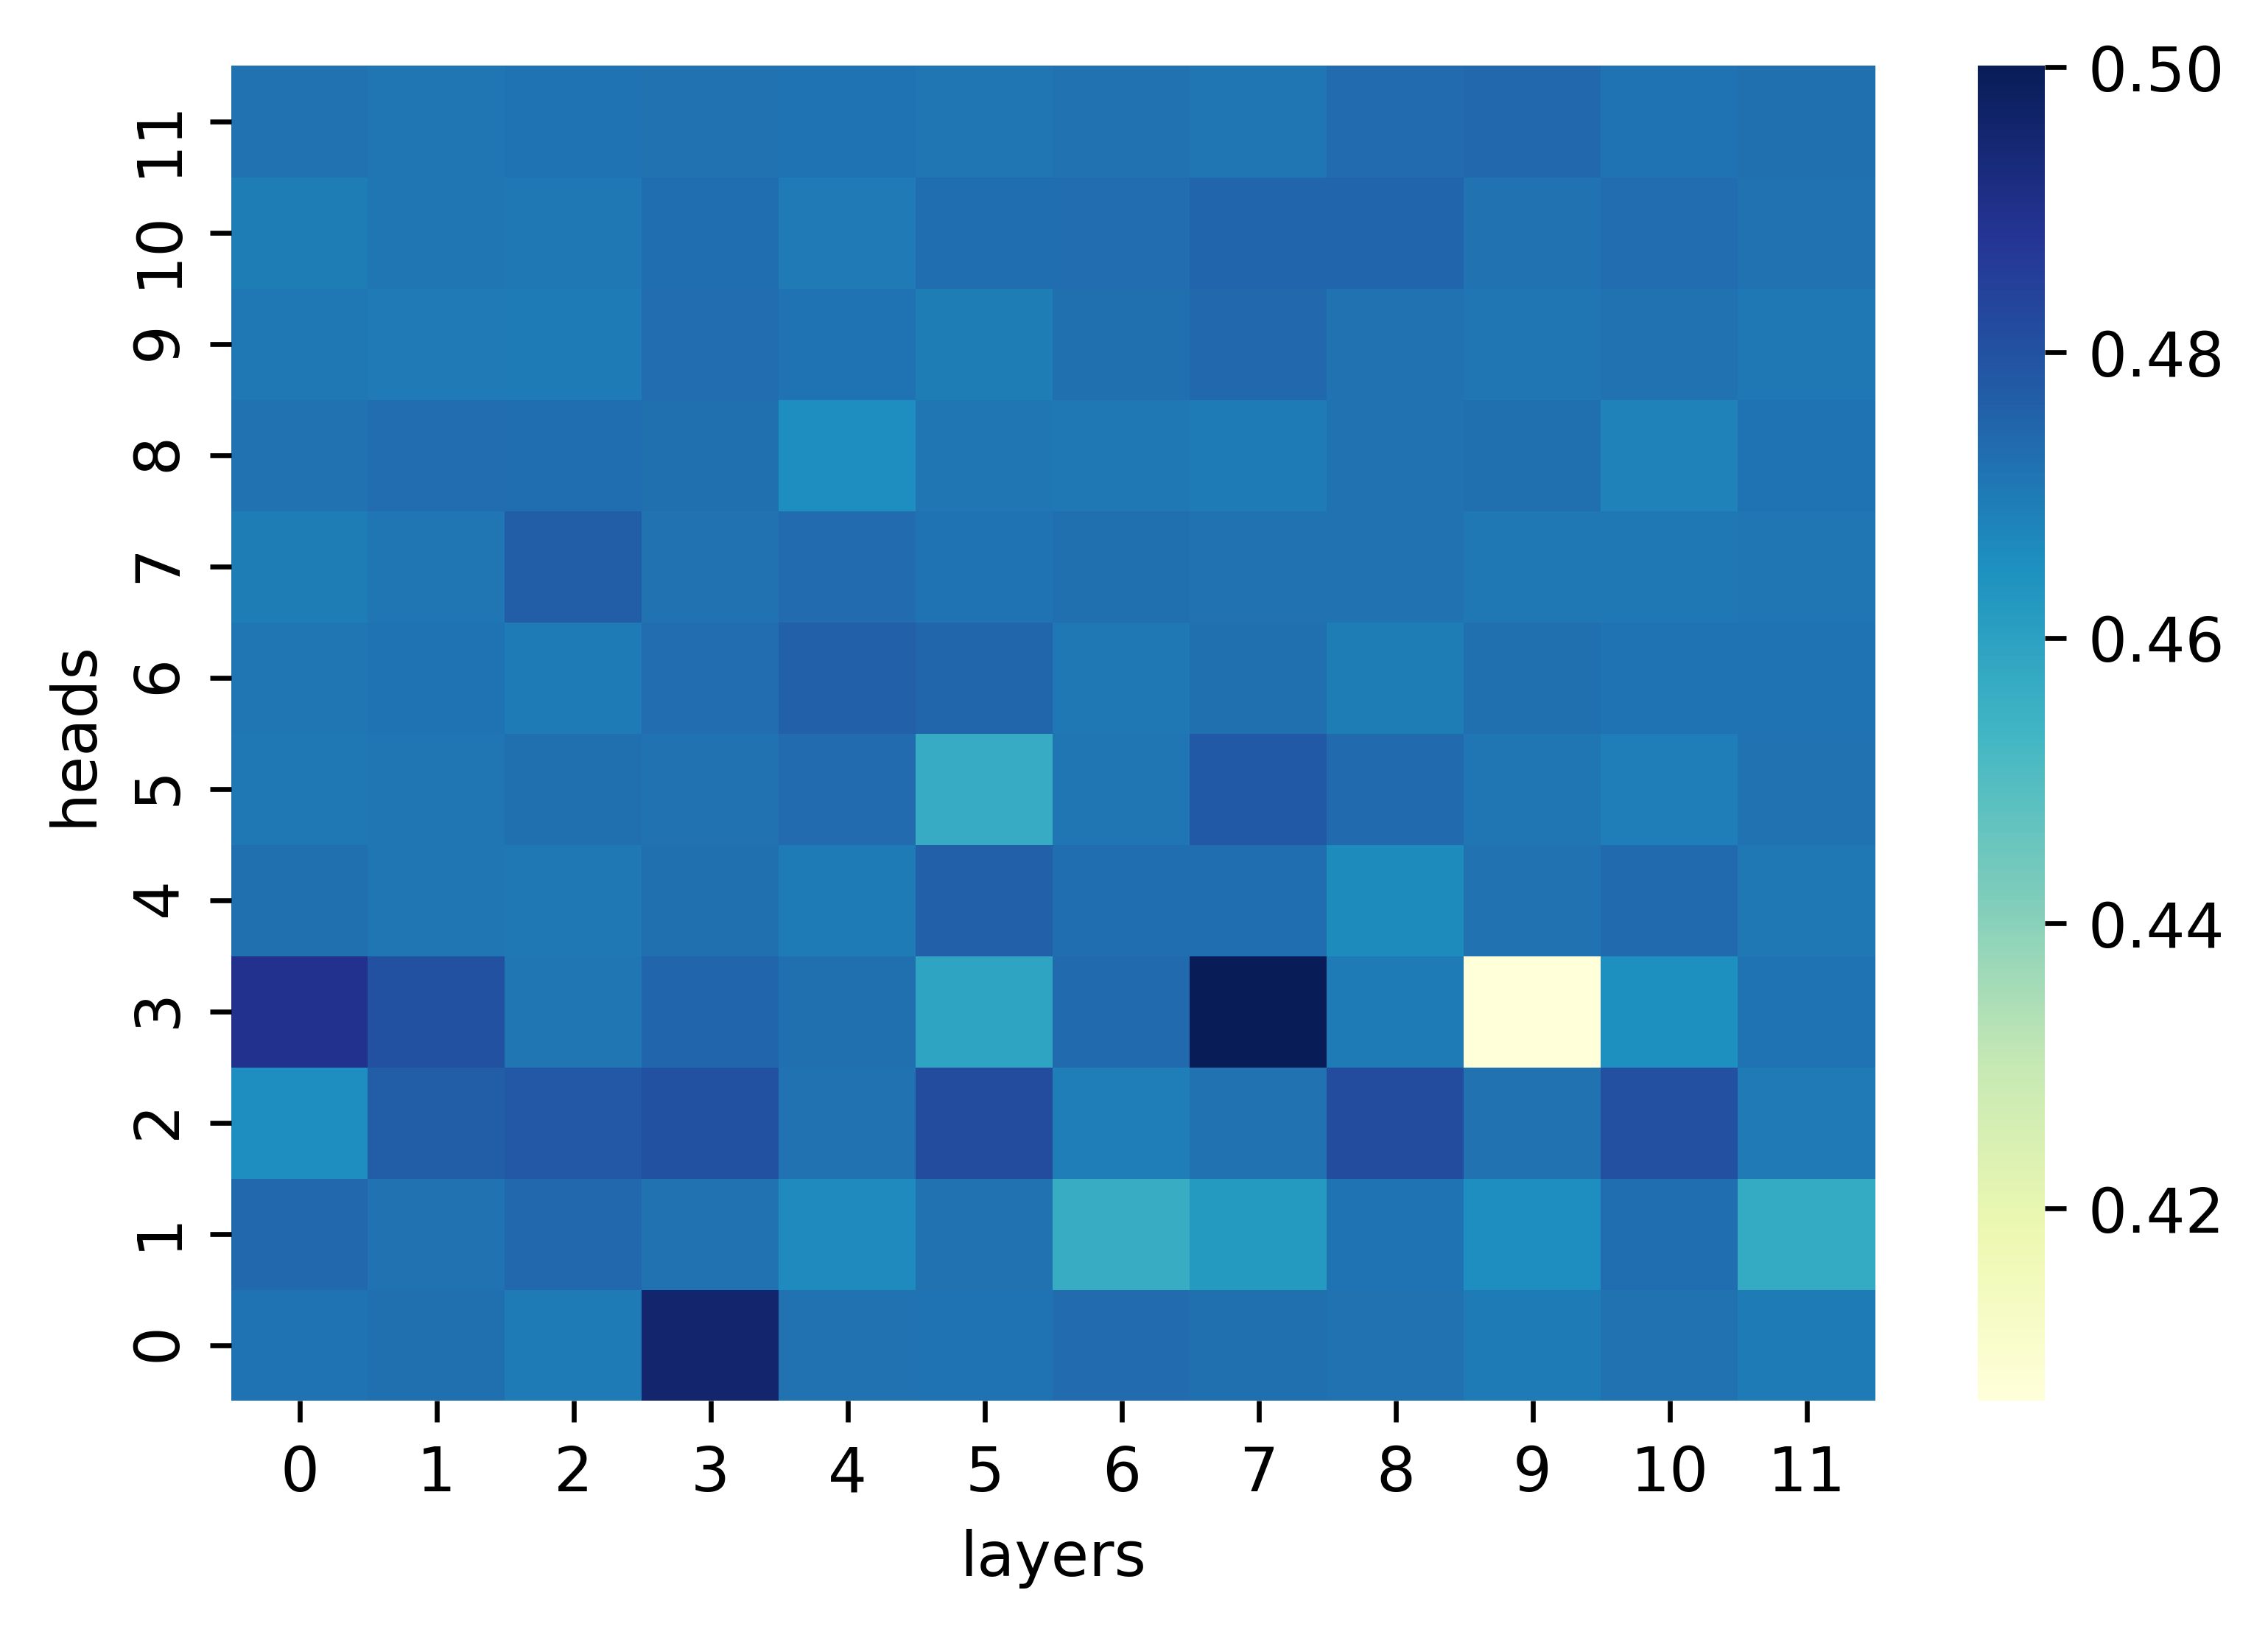
\includegraphics[width=0.75\linewidth]{heads}
			\figlabel{fig:heads}
		\end{minipage}%
	}%
	\subfigure[layers]{
		\begin{minipage}[r]{0.5\linewidth}
			\centering
			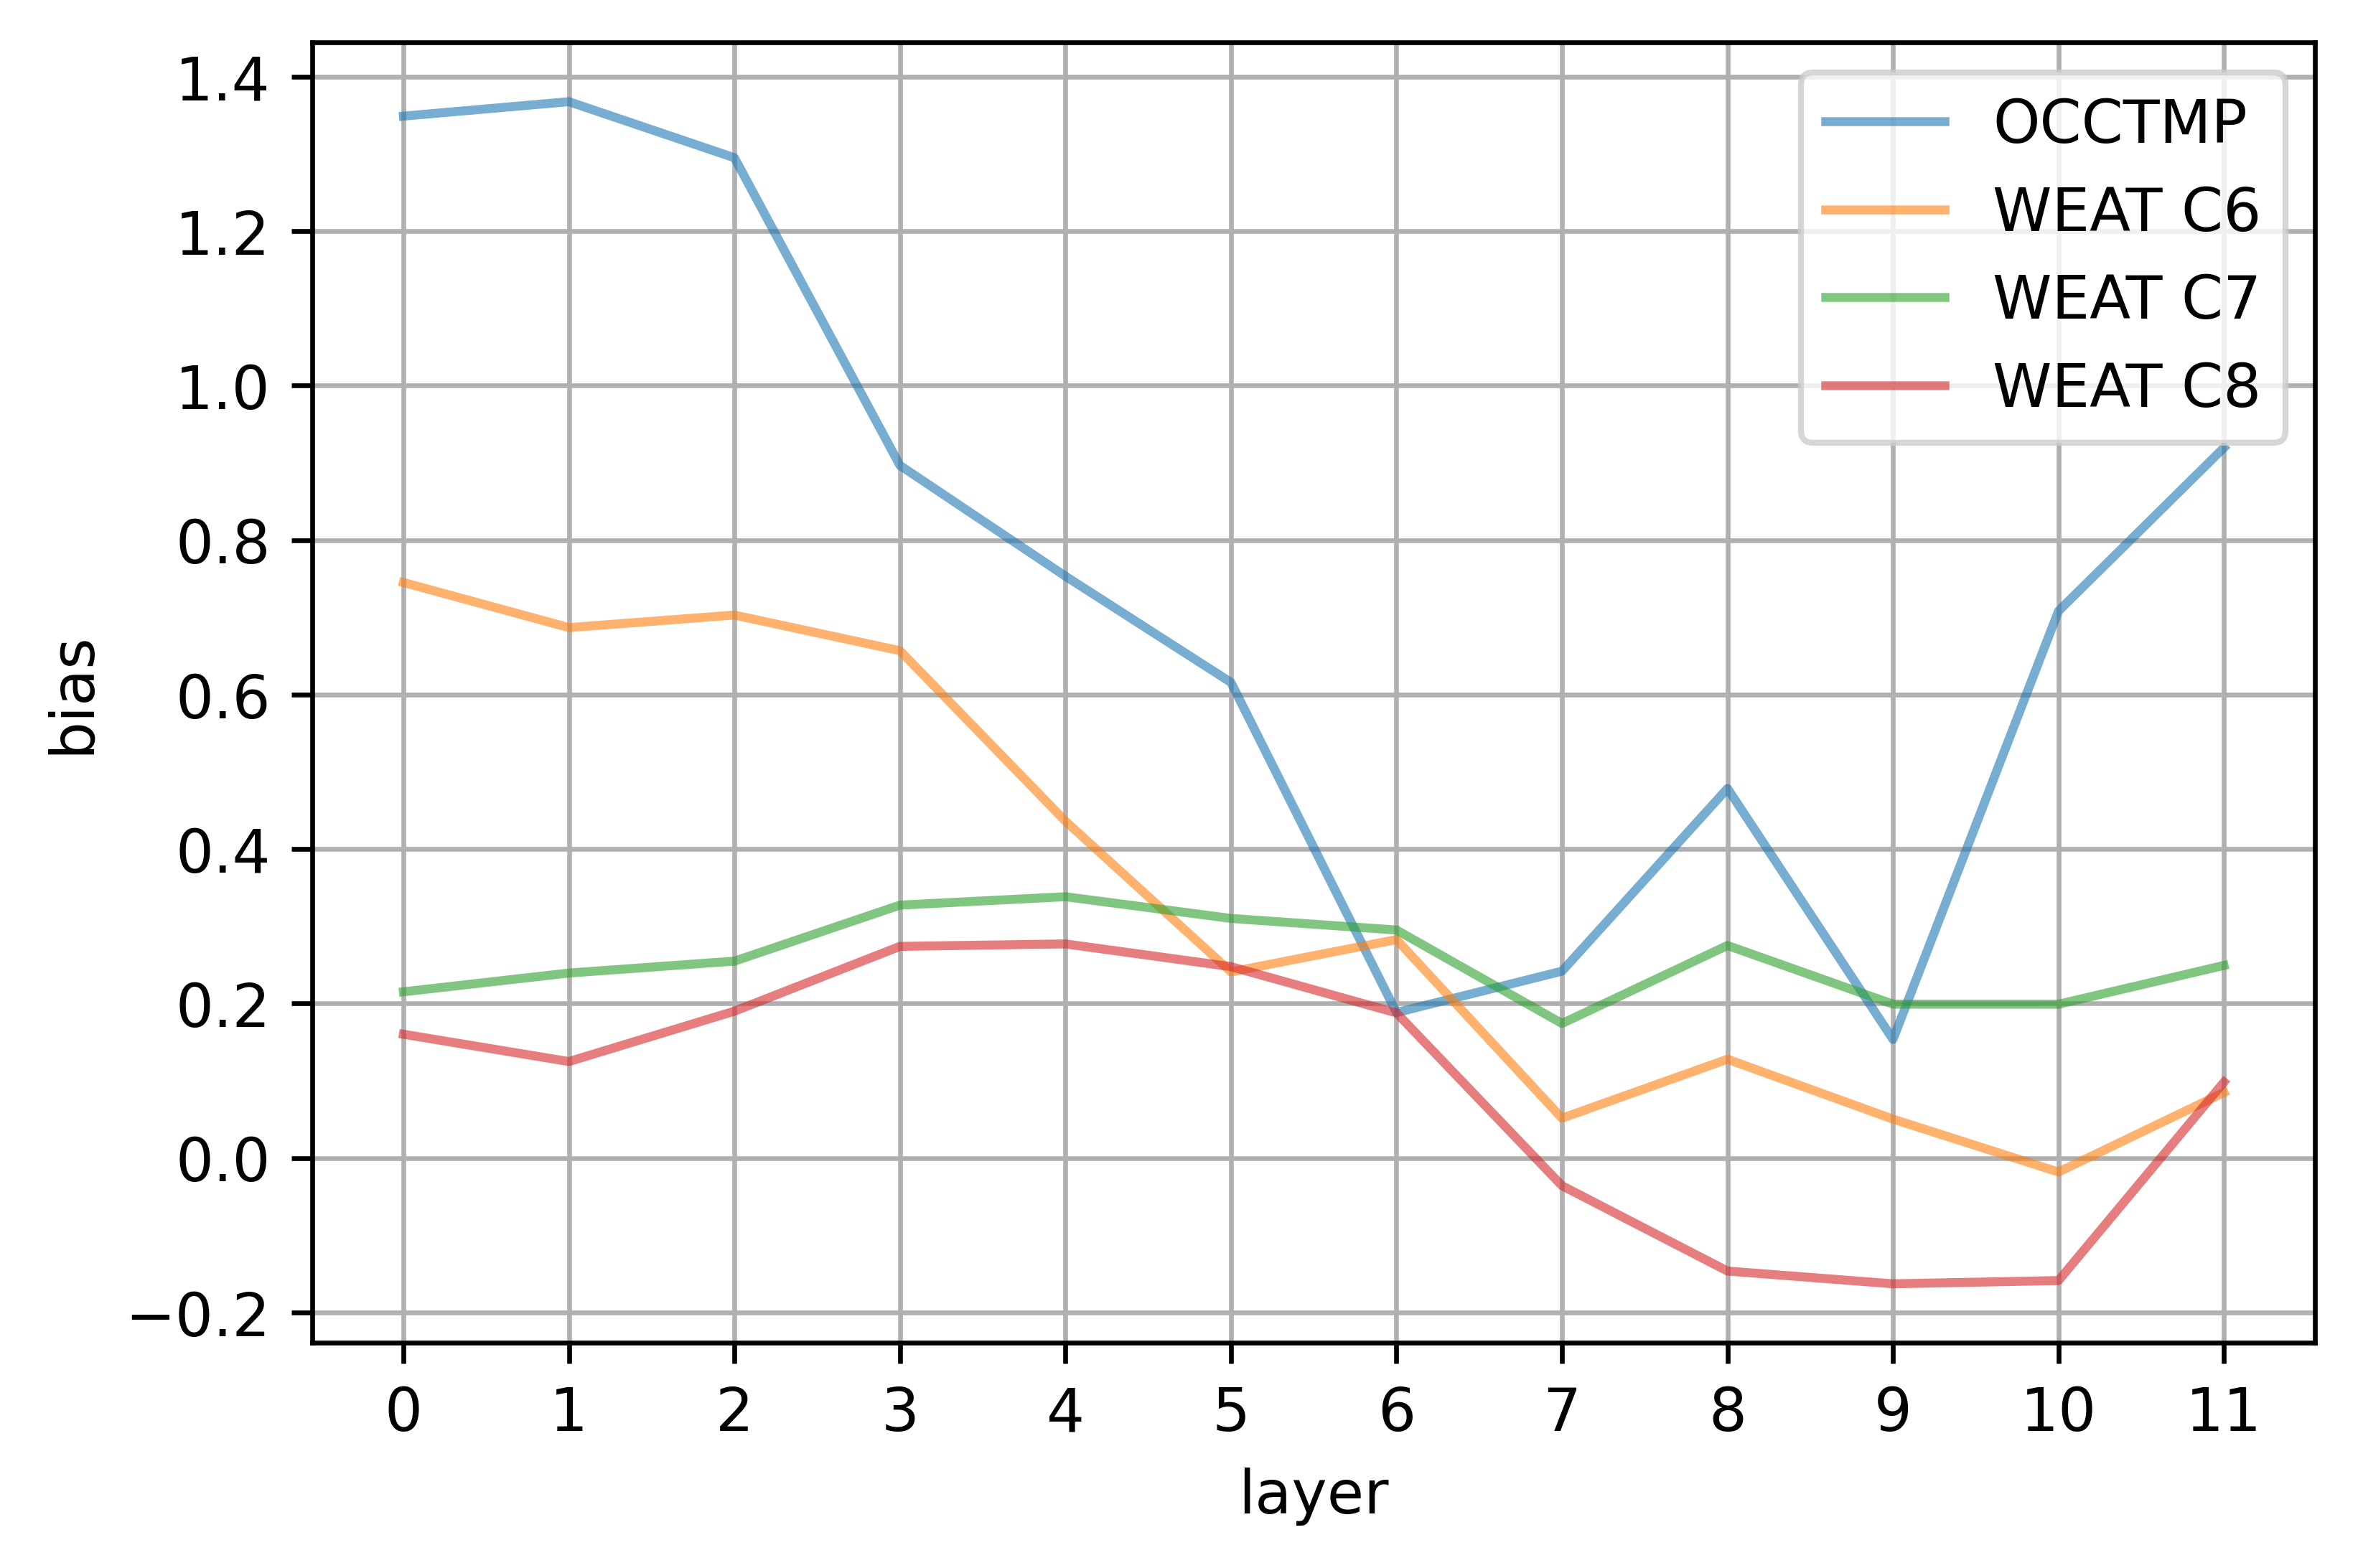
\includegraphics[width=0.75\linewidth]{layers}
			\figlabel{fig:layersbase}
		\end{minipage}%
	}%
	\centering
	\caption{(a): DensRay debiasing on each single attention head in bert-base, measured by \text{diff} on OCCTMP. (b): DensRay debiasing on each single layer, measured by \text{diff} on  OCCTMP and $d$-value on WEAT.}
	\figlabel{fig:headsandlayers}
\end{figure}

\subsubsection{Quantifying Gender Bias with DensRay}
\seclabel{quantify}
DensRay can be used to quantify gender bias for sentences
and tokens. We use the distance to the origin of the gender
subspace as the measurement. In BERT, we use the average
bias score of tokens to quantify the whole
sentence. \tabref{t:measure1} compares DensRay with the log
probability score \cite{kurita2019measuring}, which
quantifies gender bias based on templates of form ``[TARGET]
is a [ATTRIBUTE]''. We regard zero as a balance point
without bias. Contrary to the log probability score, a
positive DensRay score represents the level of female
bias. These examples show that DensRay is more versatile, it
can quantify  bias both on the token and on the sentence level.
\begin{table}[h]
	\centering
	\scriptsize
	\begin{tabular}{cccccc|c||c}
		\hline
		\multicolumn{6}{c|}{DensRay}&Avg.&log probability score\\		
		\hline\hline
		[MASK] &is &a &professor& . &&&\\
		-0.69 &-0.97 &-0.9  &-0.15  &0.45& &-0.45& 0.63\\
		\hline
		[MASK] &is &a &nurse& . &&&\\
		2.43  &1.34  &1.7   &1.93  &0.5&& 1.58 &-5.44\\
		\hline
		The &professor &asked &me& . &&&\\
		-1.25 &-0.55 &-0.08  &0.59  &0.35 &&-0.19 &
                not applicable\\
		\hline
		The &professor &asked &the&nurse &.&&\\
		-1.3&  -0.25  &0.24  &1.28  &2.19
                &0.45&0.43& not applicable\\
		\hline
	\end{tabular}
	\caption{\tablabel{t:measure1}
		Examples for quantifying bias (model: bert-base).}
\end{table}



\subsubsection{Number of Training Samples}
In the experiments, we collected training samples for DensRay by considering occurrences of the same word in the corpus across different sentences. This greatly enriches training samples. We also collected equally many masculine and feminine words for data balancing. Now we analyze the impact of these processes. DensRay is essentially a supervised learning method. It is difficult to extract useful features in the case of insufficient or unbalanced labels.  As shown in \figref{curve}, the debiasing results improve with an increased number of training samples.

As a projection-based debiasing method, the premise of DensRay debiasing is that the gender direction should be correct. Unbalanced samples will lead to incorrect gender direction biased towards either the male or the female, resulting in reversing the gender bias during debiasing. For example, if there are more masculine samples, then the embeddings will be biased towards feminine after debiasing. The figure also shows that a balanced training set improves  debiasing performance.
\begin{figure}[h]
	\centering
	\footnotesize
	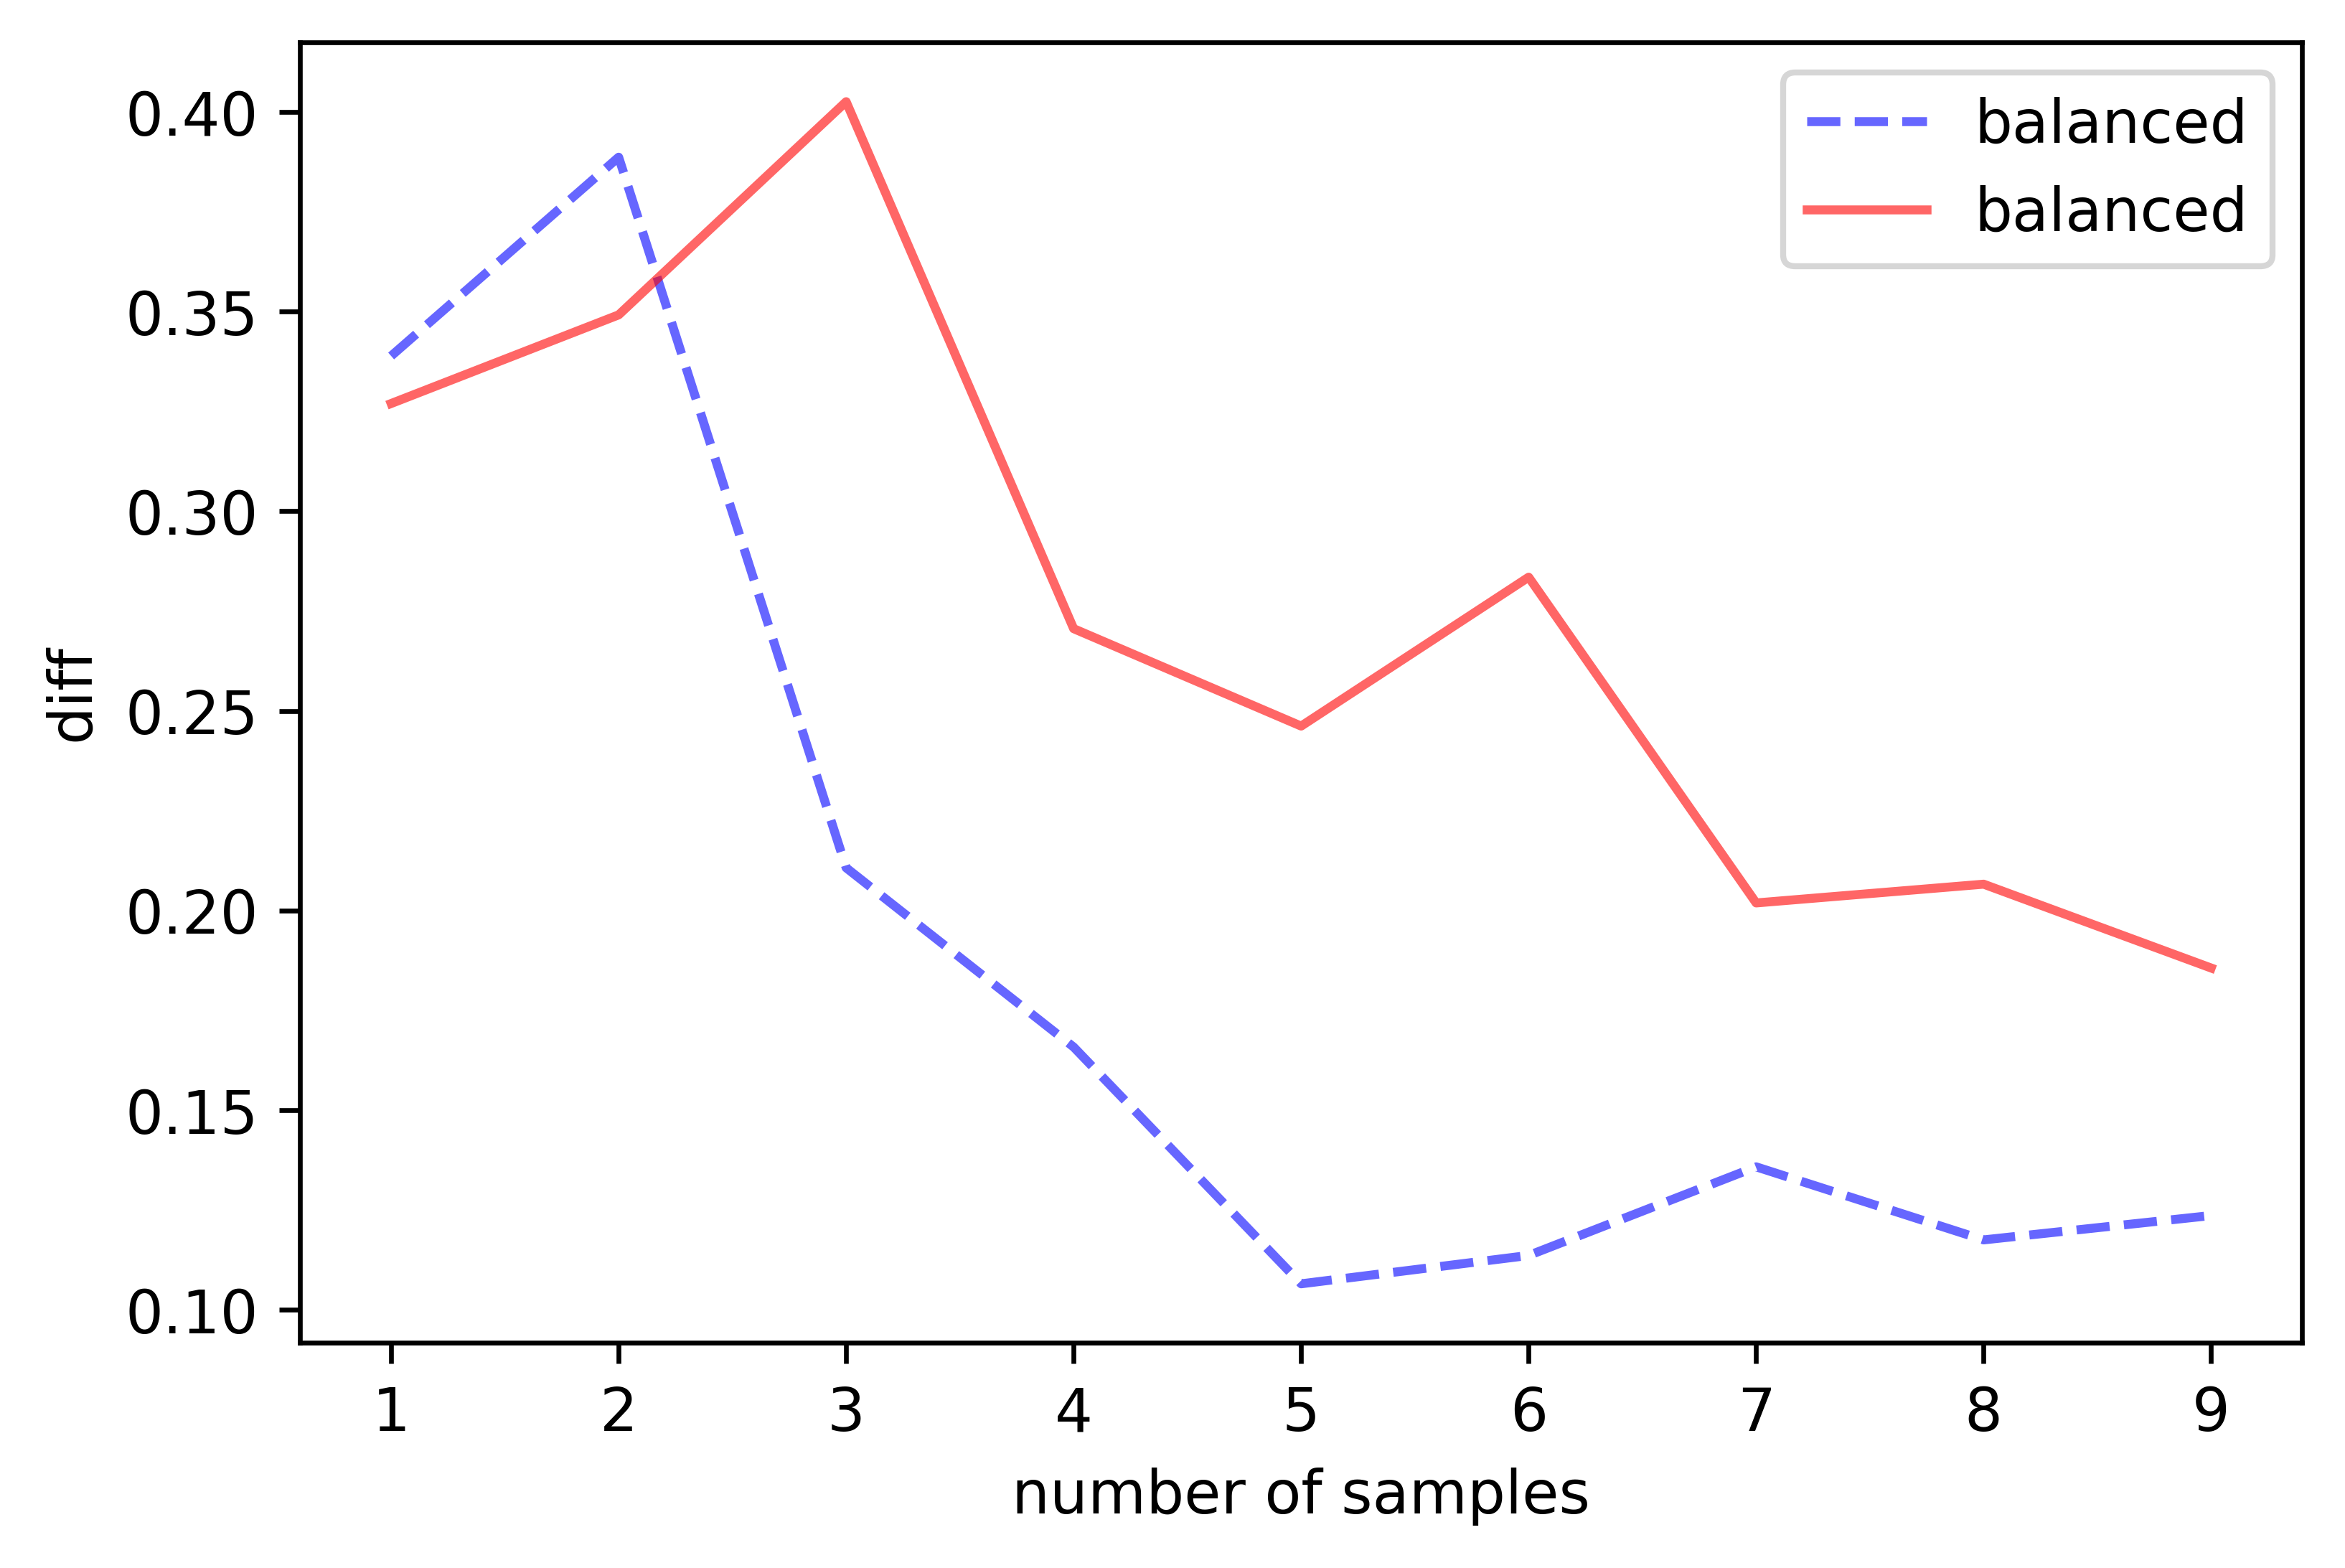
\includegraphics[width=0.4\linewidth]{samples}
	\caption{DensRay debiasing results on OCCTMP with different number of samples and unbalanced/balanced data.}
	\figlabel{curve}
\end{figure}

\subsubsection{Balancing Gender Bias}
In our experiments, we zero out the dimensions of the gender
subspace to remove gender bias. 
We also explored three alternatives to zeroing out. 1)
Replace the first dimension of the gender subspace with the
mean value of the first dimension of the training
samples. 2) Standardize the first dimension. 3) Replace the
first dimension with a small random variable sampled from a Gaussian distribution. All of them did not perform well. We further checked the mean and found that the mean of the different layers is not stable around zero, which is a problem worthy of further exploration. We also tried to delete more dimensions. However removing more dimensions does not improve the debiasing results significantly while harming the model performance.


\subsection{Multilingual Debiasing}
We now show that, in a multilingual contextualized language model like mBERT, we can use DensRay for zero-shot debiasing. Specifically, we train a DensRay model on English and use it to debias Chinese.
We use  bert-base-multilingual-uncased from
\cite{wolf2019huggingfaces}. We use the same setup as for
bert-base-uncased in our previous experiments. As before, we
compute the rotation matrices using the English gendered
words from the ``family'' category of the Google analogy
test set \cite{mikolov2013efficient}.

Since Chinese is a language that does not mark gender, we can construct the OCCTMP templates by directly translating from the English templates. We use the following form:
``\text{[MASK]}\yin{是一个}\textit{occupation}\yin{。}'' We translate the occupation using Tencent Translation\footnote{https://fanyi.qq.com/} and make some manual adjustments to the translation. After removing duplicates,  302 Chinese templates remain.

\tabref{t:templates3} gives results for the Chinese templates. Two examples are given in \tabref{t:templates3}. We see that DensRay trained with English can mitigate gender bias in mBERT: the diff score drops from 1.39 to 1.22 on Chinese templates. 
\begin{table}[h]
	\centering
	\footnotesize
	\begin{tabular}{lccccc}
		\hline
		model & prob(he) & prob(she) & sum &diff & var\\
		\hline
		 bert-multi-en 
		& 0.51 & 0.14 & 0.65 & 1.66&0.81 \\ 
		bert-multi-densray-en & 0.33 & 0.12 & 0.46 & 1.33&0.65 \\
		\hline
		 bert-multi-cn 
		& 0.24 & 0.07 & 0.31 & 1.39&0.60 \\
		 bert-multi-densray-cn 
		& 0.12 & 0.04 & 0.17 & 1.22&0.47\\
		\hline
	\end{tabular}
	\caption{\tablabel{t:templates3}
		Results of OCCTMP on mBERT after applied DensRay. Models with \textit{-en} are tested on English templates, and those with \textit{-cn} are tested on Chinese templates.}
\end{table}

\begin{table}[h]
	\centering
	\footnotesize
	\begin{tabular}{llcccc}
		\hline
		sentence & model & \yin{prob(他)} & \yin{prob(她)}&sum&diff\\
		\hline
		\yin{\text{[MASK]}是一个客座教授。} & bert-multi-en & 0.68 & 0.16&0.84&1.45\\
		\text{[MASK]} is an adjunct professor.& bert-multi-densray-en & 0.51 & 0.18&0.70&1.04\\
		& bert-multi-cn & 0.52 & 0.11&0.63&1.55\\
		& bert-multi-densray-cn & 0.30 & 0.08&0.38&1.31\\
		\hline
		\yin{\text{[MASK]}是一个管理员。} & bert-multi-en & 0.53 & 0.17&0.70&1.14\\
		\text{[MASK]}is an administrator.& bert-multi-densray-en & 0.35 & 0.13&0.48&0.99\\
		& bert-multi-cn & 0.68 & 0.16&0.84&1.45\\
		& bert-multi-densray-cn & 0.51 & 0.18&0.69&1.04\\
		\hline
	\end{tabular}
	\caption{\label{t:templates3}
		Sanity check on the Chinese templates, where \yin{\textit{他}} means \textit{he} and \yin{\textit{她}} means \textit{she}. Corresponding English translations are shown below the Chinese.}
\end{table}
